
\documentclass[hyperref={pdfpagelabels=false},ngerman]{beamer}

% stop font warning
\let\Tiny=\tiny
\providecommand\thispdfpagelabel[1]{}

\usepackage[english]{babel}
\usepackage{lmodern}
\usepackage[T1]{fontenc}
\usepackage[utf8]{inputenc}
\usepackage{graphicx,import}
\usepackage{feynmp}
\DeclareGraphicsRule{*}{mps}{*}{} 
\DeclareGraphicsExtensions{.pdf}
\usepackage{amsmath,amssymb,amstext,amsfonts} % mathrsfs
\usepackage{array,booktabs,tabularx}
\usepackage{tikz,tikz-uml,pgf-pie}
\usetikzlibrary{shapes,calc,arrows,positioning}
\tikzstyle{block} = [rectangle, draw, text width=7em, text centered, minimum height=2em]
\tikzstyle{arrow} = [draw, -latex, thick]
\tikzstyle{arrow2} = [draw, latex-latex, thick]
\tikzstyle{quark}  = [rectangle, draw, fill=yellow, minimum width=2em, text centered, minimum height=2em]
\tikzstyle{lepton} = [rectangle, draw, fill=red!50, minimum width=2em, text centered, minimum height=2em]
\tikzstyle{gauge}  = [circle   , draw, fill=green , minimum size=2em, inner sep=0pt, text centered]
\tikzstyle{scalar} = [diamond  , draw, fill=blue!40, minimum width=2.3em, text centered, minimum height=2.3em, inner sep=0pt]
\tikzstyle{goldstone} = [diamond, draw, dashed, fill=blue!30, minimum width=2.3em, text centered, minimum height=2.3em, inner sep=0pt]
\tikzstyle{squark}   = [diamond, draw, fill=yellow, minimum width=2.3em, text centered, minimum height=2.3em, inner sep=0pt]
\tikzstyle{slepton}  = [diamond, draw, fill=red!50, minimum width=2.3em, text centered, minimum height=2.3em, inner sep=0pt]
\tikzstyle{gaugino}  = [rectangle, draw, fill=green , minimum size=2em, inner sep=0pt, text centered]
\tikzstyle{higgsino} = [rectangle, draw, fill=blue!40  , minimum width=2em, text centered, minimum height=2em]
\tikzstyle{inert}    = [diamond  , draw, fill=teal!80, minimum width=2.3em, text centered, minimum height=2.3em, inner sep=0pt]
\tikzstyle{inertino} = [rectangle, draw, fill=teal!80, minimum width=2em, text centered, minimum height=2em]
\tikzstyle{phantom}  = [rectangle, minimum width=2em, text centered, minimum height=2em]
\usepackage{slashed}
\usepackage{fixltx2e} % textsubscript
\usepackage{multirow}
\usepackage{tcolorbox}
\usepackage{pifont}
\usepackage{xspace}
\usepackage{hyperref}
\hypersetup{colorlinks,linkcolor=,urlcolor=blue}
\usepackage{listings}
\lstset{breaklines=true,
  breakatwhitespace=true,
%  numbers=left,
  numberstyle=\tiny,
  stepnumber=1,
  basicstyle=\ttfamily\footnotesize,
  commentstyle=\ttfamily\color{gray},
  postbreak={\mbox{{$\hookrightarrow$}}\space\space},
  breakindent=10pt,
  breakautoindent=false,
  showspaces=false,
  showstringspaces=false,
  frame=single}

\definecolor{darkgreen}{RGB}{0,176,0}

\newcommand{\cmark}{\ding{51}}%
\newcommand{\xmark}{\ding{55}}%
\newcommand{\fmfvcenter}[1]{\;\vcenter{\hbox{\fmfreuse{#1}}}\;}
\newcommand{\eh}[1]{\,\mathsf{#1}}
\newcommand{\ok}{\textcolor{darkgreen}{\cmark}}
\newcommand{\notok}{\textcolor{red}{\xmark}}
\newcommand{\maybe}{\textcolor{gray}{\cmark}}
\newcommand{\meh}{\textcolor{gray}{\textbf{\huge\lower.1em\hbox{-}}}}
\newcommand{\Lagr}{\mathcal{L}}
\newcommand{\MS}{\ensuremath{M_S}}
\newcommand{\mathi}{\mathsf{i}}
\newcommand{\mycite}[1]{\ensuremath{\text{\textcolor{darkgray}{\tiny [#1]}}}}
\newcommand{\bigcite}[1]{\textcolor{darkgray}{[#1]}}
\newcommand{\dimrep}[1]{\mathbf{#1}}
\newcommand{\dimrepadj}[1]{\mathbf{\overline{#1}}}
\newcommand{\ESSM}{E\textsubscript{6}SSM}
\newcommand{\CESSM}{CE\textsubscript{6}SSM}
\DeclareMathOperator{\tildeRe}{\widetilde Re}
\DeclareMathOperator{\sign}{sign}
\DeclareMathOperator{\re}{Re}
\DeclareMathOperator{\im}{Im}
\renewcommand{\emph}[1]{\textbf{\textcolor{darkblue}{#1}}}
\newcommand{\dd}{\mathsf{d}}
\newcommand{\myurl}[1]{\href{#1}{#1}}
\newcommand{\Superpot}{\mathcal{W}}
\newcommand{\SuperField}[1]{#1}
\newcommand{\ConjSuperField}[1]{\bar{#1}}
\newcommand{\UY}{\ensuremath{U(1)_{Y}}}
\newcommand{\UN}{\ensuremath{U(1)_{N}}}
\newcommand{\Uem}{\ensuremath{U(1)_\text{em}}}
\newcommand{\SUL}{\ensuremath{SU(2)_\text{L}}}
\newcommand{\SUc}{\ensuremath{SU(3)_\text{c}}}
\newcommand{\SOten}{\ensuremath{{SO(10)}}}
\newcommand{\comma}{,}
\newcommand{\DRbar}{\ensuremath{\overline{\text{DR}}}}
\newcommand{\DRbarp}{\ensuremath{\overline{\text{DR}}'}}
\newcommand{\MSbar}{\ensuremath{\overline{\text{MS}}}}
\newcommand{\SM}{\ensuremath{\text{SM}}}
\newcommand{\MSSM}{\ensuremath{\text{MSSM}}}
\newcommand{\BSM}{\ensuremath{\text{BSM}}}
\newcommand{\pole}{\ensuremath{\text{pole}}}
\newcommand{\tree}{\ensuremath{\text{tree}}}
\newcommand{\fsstar}{\textbf{*}}
\newcommand{\FS}{\texttt{FlexibleSUSY}\xspace}
\newcommand{\fsh}{\texttt{FS+H}\xspace}
\newcommand{\feft}{\texttt{FlexibleEFTHiggs}\xspace}
\newcommand{\hssusy}{\texttt{HSSUSY}\xspace}
\newcommand{\Himalaya}{\texttt{Himalaya}\xspace}
\newcommand{\FH}{\texttt{FeynHiggs}\xspace}
\newcommand{\SPheno}{\texttt{SPheno}\xspace}
\newcommand{\SARAH}{\texttt{SARAH}\xspace}
\newcommand{\SOFTSUSY}{\texttt{SOFTSUSY}\xspace}
\newcommand{\Zv}{\ensuremath{\backslash\mkern-11.0mu{Z_3}}}
\newcommand{\downrightknickarrow}{\mathrel{\scalebox{1.3}{\rotatebox[origin=c]{180}{$\Lsh$}}}}
\newcommand{\threelinebrace}{$\left. \begin{array}{c} \\ \\ \\ \end{array} \right\rbrace$}
\newcommand{\fivelinebrace}{$\left. \begin{array}{c} \\ \\ \\ \\ \\ \end{array} \right\rbrace$}
\newcommand{\twolinebrace}{$\left. \begin{array}{c} \\ \\ \end{array} \right\rbrace$}
\newcommand{\elevenlinebrace}{$\left. \begin{array}{c} \\ \\ \\ \\ \\ \\ \\ \\ \\ \\ \\ \end{array} \right\rbrace$}
\newcommand{\at}{\alpha_t}
\newcommand{\ab}{\alpha_b}
\newcommand{\atau}{\alpha_\tau}
\newcommand{\as}{\alpha_s}
\newcommand{\aem}{\alpha_\text{em}}
\newcommand{\GeV}{\eh{GeV}}
\newcommand{\TeV}{\eh{TeV}}
\newcommand{\SQCD}{\ensuremath{\scalefont{.8}\text{SQCD}}}
\newcommand{\Qpole}{\ensuremath{Q_\text{pole}}}
\newcommand{\Qmatch}{\ensuremath{Q_\text{match}}}
\newcommand{\DMh}{\ensuremath{\Delta M_h^{(\text{FO})}}}
\newcommand{\DMhQpole}{\ensuremath{\Delta M_h^{(\Qpole)}}}
\newcommand{\DMhQmatch}{\ensuremath{\Delta M_h^{(\Qmatch)}}}
\newcommand{\DMhMt}{\ensuremath{\Delta M_h^{(m_t)}}}
\newcommand{\DMhAlphaS}{\ensuremath{\Delta M_h^{(\as)}}}
\newcommand{\DMhAlphaEm}{\ensuremath{\Delta M_h^{(\aem)}}}
\newcommand{\DMhHSSUSY}{\ensuremath{\Delta M_h^{(\text{EFT})}}}
\newcommand{\DMhHSSUSYytSM}{\ensuremath{\Delta M_h^{(y_t^\SM)}}}
\newcommand{\DMhHSSUSYytMSSM}{\ensuremath{\Delta M_h^{(y_t^\MSSM)}}}
\newcommand{\DMhEFT}{\ensuremath{\Delta M_h^{(v^2/\MS^2)}}}
\def\HSSUSY{\texttt{HSSUSY}}

% set look of slides
\usetheme{Madrid}
\useoutertheme{default}
\useinnertheme{circles}
\usecolortheme{default}
\beamertemplatenavigationsymbolsempty % keine Navigationselemente
\setbeamersize{text margin left = 1cm, text margin right = 1cm}

% define footer
\makeatletter
\setbeamertemplate{footline}
{
  \hfill\hbox{\insertframenumber{} / \inserttotalframenumber\hspace*{4pt}}%
  \vskip3pt%
}
\makeatother
\usecolortheme{tud}

\title{Precise Higgs mass predictions in the (N)MSSM}

\author[Alexander Voigt]{Alexander Voigt}

\date{SUSY-2018\\[1em]
  23--27/07/2018}

% \institute[Aachen]{RWTH Aachen}
\subject{FlexibleSUSY,MSSM,Higgs,FlexibleEFTHiggs}
\keywords{FlexibleSUSY,MSSM,Higgs,FlexibleEFTHiggs}

%%%%%%%%%%%%%%%%%%%%%%%%%%%%%%%%%%%%%%%%%%%%%%%%%%%%%%%%%%%%%%%%%%%%%%%%%%%%%

\begin{document}

%%%%%%%%%%%%%%%%%%%%%%%%%%%%%%%%%%%%%%%%%%%%%%%%%%%%%%%%%%%%%%%%%%%%%%%%%%%%%

% Savebox which contains the the Feynman rules
\newsavebox{\feynmanrules}
\sbox{\feynmanrules}{
\begin{fmffile}{Feynman/higgs} % file name and path
  \fmfset{thin}{.8pt}
  \fmfset{wiggly_len}{5mm}
  \fmfset{dash_len}{2.5mm}
  \fmfset{dot_size}{1thick}
  \fmfset{arrow_len}{2.5mm}
  \fmfset{curly_len}{2.5mm}

\begin{fmfgraph*}(60,60)
  \fmfkeep{hX}
  \fmfleft{v1}
  \fmfright{v2}
  \fmf{higgs}{v1,c1}
  \fmf{higgs}{c2,v2}
  \fmf{quark,left,tension=0.5,label=$X$}{c1,c2}
  \fmf{quark,left,tension=0.5}{c2,c1}
\end{fmfgraph*}

\begin{fmfgraph*}(60,60)
  \fmfkeep{htop}
  \fmfleft{v1}
  \fmfright{v2}
  \fmf{higgs}{v1,c1}
  \fmf{higgs}{c2,v2}
  \fmf{quark,left,tension=0.5,label=$t$}{c1,c2}
  \fmf{quark,left,tension=0.5}{c2,c1}
\end{fmfgraph*}

\begin{fmfgraph*}(60,60)
  \fmfkeep{hstop}
  \fmfleft{v1}
  \fmfright{v2}
  \fmf{higgs}{v1,c1}
  \fmf{higgs}{c2,v2}
  \fmf{scalar,left,tension=0.5,label=$\tilde{t}_i$}{c1,c2}
  \fmf{scalar,left,tension=0.5}{c2,c1}
\end{fmfgraph*}

\begin{fmfgraph*}(60,60)
  \fmfkeep{hstopA}
  \fmfleft{v1}
  \fmfright{v2}
  \fmf{higgs}{v1,c,v2}
  \fmf{scalar,right,tension=0.8,label=$\tilde{t}_i$}{c,c}
\end{fmfgraph*}

\begin{fmfgraph*}(60,60)
  \fmfkeep{htoptad}
  \fmfleft{v1}
  \fmfright{v2}
  \fmftop{t1}
  \fmf{higgs}{v1,c,v2}
  \fmffreeze
  \fmf{higgs}{c,c1}
  \fmf{quark,right,tension=0.3,label=$t$}{c1,c2}
  \fmf{quark,right,tension=0.3}{c2,c1}
  \fmf{phantom,tension=10}{c2,t1}
\end{fmfgraph*}

\begin{fmfgraph*}(60,60)
  \fmfkeep{hstoptad}
  \fmfleft{v1}
  \fmfright{v2}
  \fmftop{t1}
  \fmf{higgs}{v1,c,v2}
  \fmffreeze
  \fmf{higgs}{c,c1}
  \fmf{scalar,right,tension=0.3,label=$\tilde{t}_i$}{c1,c2}
  \fmf{scalar,right,tension=0.3}{c2,c1}
  \fmf{phantom,tension=10}{c2,t1}
\end{fmfgraph*}
\end{fmffile}
}

%%%%%%%%%%%%%%%%%%%%%%%%%%%%%%%%%%%%%%%%
\begin{frame}[plain]
  \tikz [remember picture,overlay]
  \node at
    ([yshift=1.3cm,xshift=4cm]current page.south)
    {\includegraphics[height=2cm]{images/RWTH_Logo}};
  \titlepage  
\end{frame}

%%%%%%%%%%%%%%%%%%%%%%%%%%%%%%%%%%%%%%%%
\begin{frame}{Contents}
  \tableofcontents
\end{frame}

%%%%%%%%%%%%%%%%%%%%%%%%%%%%%%%%%%%%%%%%

% \begin{frame}{Current limits on SUSY particle masses}
%   \begin{center}
%     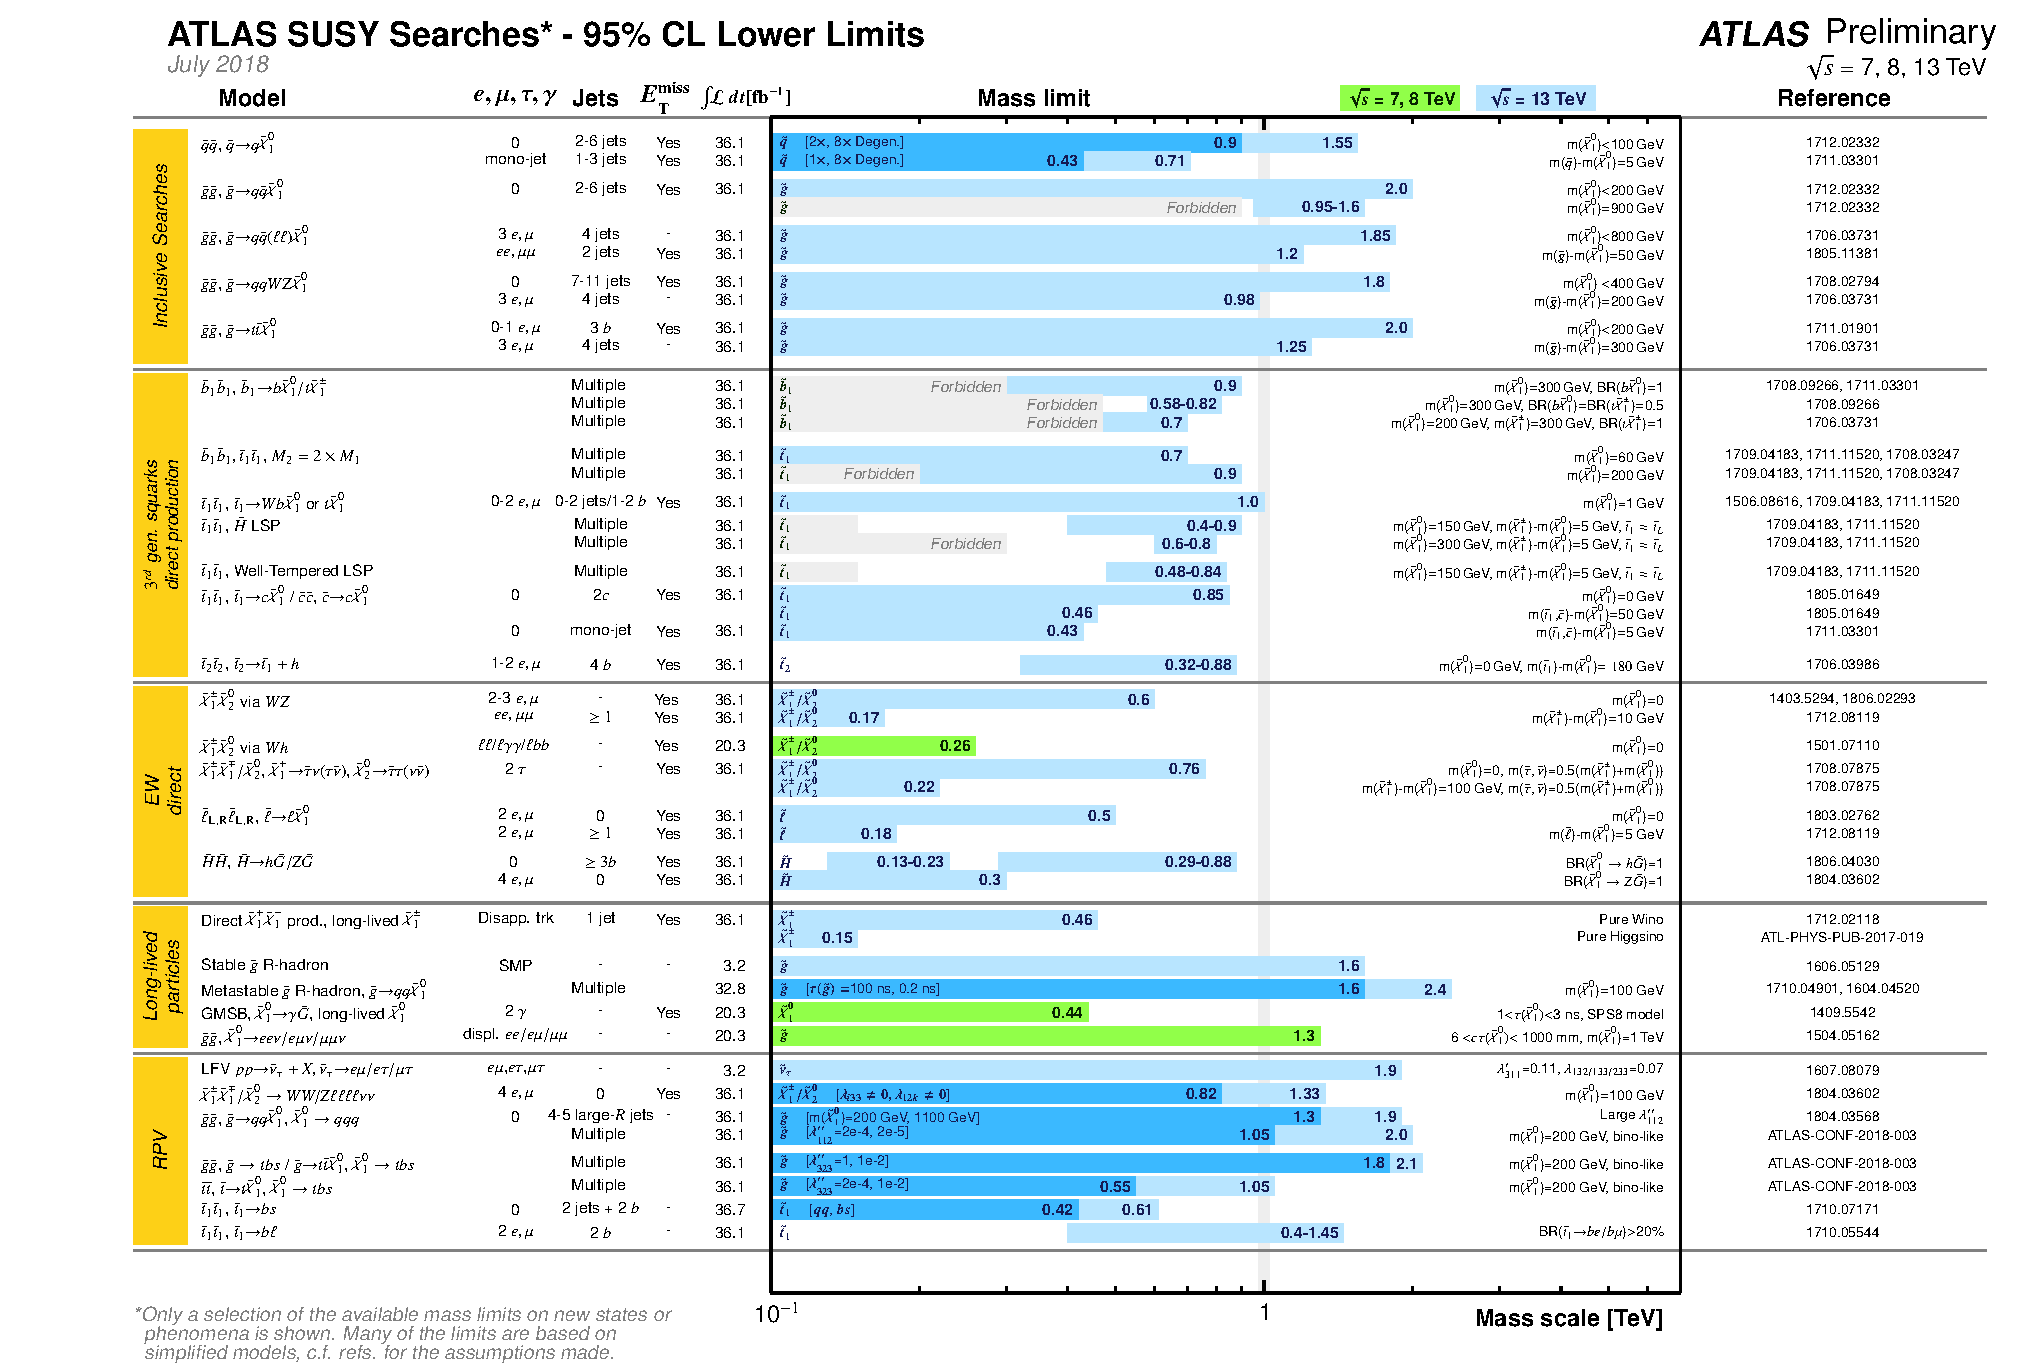
\includegraphics[width=\textwidth]{images/ATLAS_SUSY_Summary}
%   \end{center}
% \end{frame}

\section{Fixed-order calculation}
\subsection{3-loop contribution}

\begin{frame}{Contents}
  \tableofcontents[
  currentsection]
\end{frame}

\begin{frame}{Higgs mass calculation at fixed loop order in \DRbarp}
  \begin{center}
    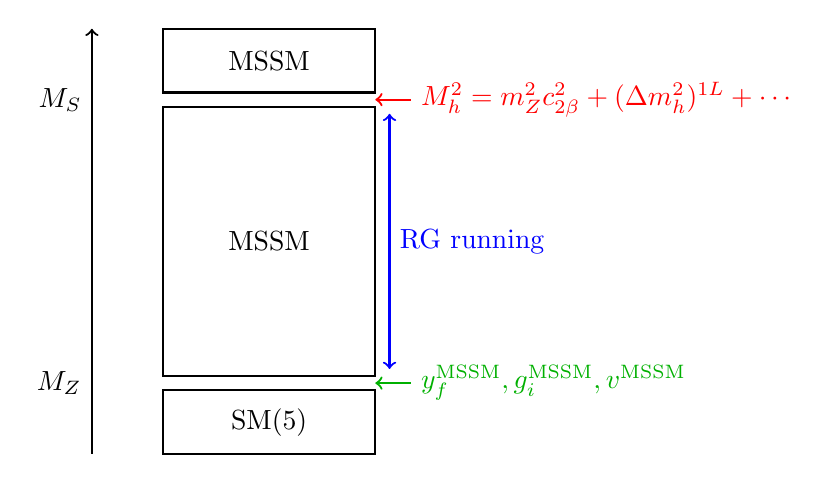
\begin{tikzpicture}[scale=0.9]
      \draw[->, thick] (0,0) -- (0,1) node[left]{$M_Z$} -- (0,5) node[left]{$\MS$} -- (0,6);
      \draw[thick] (1,0)   rectangle node{SM(5)} (4,0.9);
      \draw[thick] (1,1.1) rectangle node{MSSM}  (4,4.9);
      \draw[thick] (1,5.1) rectangle node{MSSM}  (4,6);
      \draw[<-, thick, red] (4,5) -- (4.5,5) node[right]{$M_h^2 = m_Z^2 c_{2\beta}^2 + (\Delta m_h^2)^{1L} + \cdots$};
      \draw[<-, thick, darkgreen] (4,1) -- (4.5,1) node[right]{$y_f^\MSSM, g_i^\MSSM, v^\MSSM$};
      \draw[<->, thick, blue] (4.2,1.2) -- node[right]{RG running} (4.2,4.8);
    \end{tikzpicture}
  \end{center}
\end{frame}

\begin{frame}{Known/unknown fixed order \DRbarp\ loop corrections}
  Loop corrections in the determination of the running MSSM
    parameters $y_f^\MSSM$, $g_i^\MSSM$:
    \begin{align*}
      y_t^\MSSM &= \frac{\sqrt{2}\,M_t}{v_u}
      \Big[1 + \hbar(\textcolor{darkgreen}{\text{full}})
      + \hbar^2(\textcolor{darkgreen}{\as^2} + \textcolor{red}{\at\as} + \textcolor{red}{\at^2})
      + \cdots \Big] \\
      \as^\MSSM &= \as^{\SM(5)}
      \Big[1 + \hbar(\textcolor{darkgreen}{\text{full}})
      + \hbar^2(\textcolor{darkgreen}{\as^2} + \textcolor{darkgreen}{\at\as} + \textcolor{darkgreen}{\ab\as})
      + \cdots \Big]
    \end{align*}
    \mycite{0210258, 0507139, 0707.0650, 0509048, 0810.5101, 1009.5455}\\[0.5em]
    Loop corrections to $M_h^2$ in the MSSM:
    \begin{align*}
      M_h^2 &= m_h^2 + \hbar(\textcolor{darkgreen}{\text{full}})
      + \hbar^2\Big[ m_t^2(\textcolor{darkgreen}{\at\as} + \textcolor{darkgreen}{\at^2} + \cdots)
      + \textcolor{red}{m_Z^2\aem^2}
      + \cdots\Big]\\
      &\quad + \hbar^3\Big[ m_t^2(\textcolor{darkgreen}{\underline{\at\as^2}} + \textcolor{red}{\at^2\as} + \textcolor{red}{\at^3})
      + \cdots\Big]
    \end{align*}
    \mycite{0105096, 0112177, 0212132, 0206101, 0305127, 1005.5709, \underline{1708.05720}, \underline{1807.03509}}
\end{frame}

\begin{frame}{Effect of the 3-loop $O(\at\as^2)$ corrections to $M_h$}
  \begin{center}
    \includegraphics[width=0.49\textwidth]{plots/SOFTSUSY/Mh_2L_vs_3L_MS_TB-20_Xt--sqrt6}\hfill
    \includegraphics[width=0.49\textwidth]{plots/Mh3L/scan_Mh_MS_TB-20_Xt--sqrt6_uncertainty_Qpole}
  \end{center}
  \mycite{1708.05720}
\end{frame}

\subsection{Uncertainty estimate}

\begin{frame}{Uncertainty estimate of the fixed-order \DRbarp\ calculation}
  In \bigcite{1804.09410} 5 sources of uncertainty were combined:
  \begin{align*}
    \DMhQpole &= \max_{\Qpole\in[\MS/2,2\MS]}\left|M_h(\Qpole) - M_h(\MS)\right| & \text{\mycite{1609.00371}} \\
    \DMhQmatch &= \max_{\Qmatch\in[M_Z/2,2M_Z]}\left|M_h(\Qmatch) - M_h(M_Z)\right| & \text{\mycite{\underline{1804.09410}}} \\
    \DMhMt &= \left|M_h(m_t^{[1]}) - M_h(m_t^{[2]})\right| & \text{\mycite{1609.00371}} \\
    \DMhAlphaS &= \left| M_h(\as^{[1]}) - M_h(\as^{[2]}) \right| & \text{\mycite{\underline{1804.09410}}} \\
    \DMhAlphaEm &= \left| M_h(\aem^{[1]}) - M_h(\aem^{[2]}) \right| & \text{\mycite{\underline{1804.09410}}}
  \end{align*}
  Combination:
  \begin{align*}
    \DMh &= \DMhQpole + \DMhQmatch + \DMhMt + \DMhAlphaS + \DMhAlphaEm 
  \end{align*}
\end{frame}

\begin{frame}{Uncertainty estimate of the fixed-order \DRbarp\ calculation}
  \begin{center}
    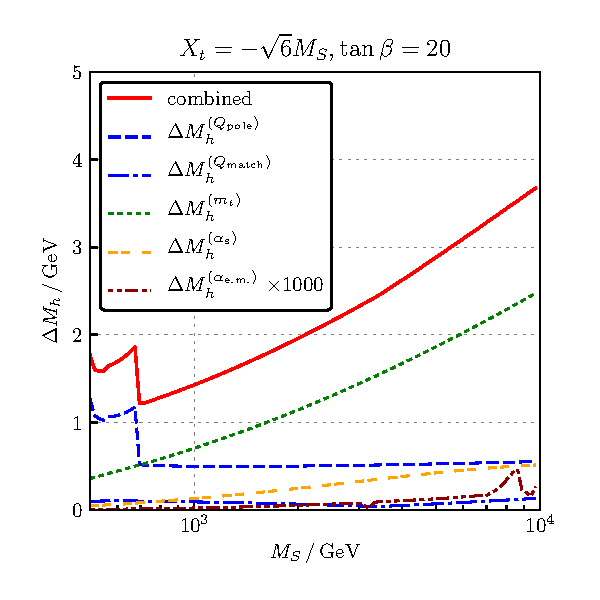
\includegraphics[width=0.49\textwidth]{{{plots/SOFTSUSY/SS_TB-20_Xt--sqrt6_individual}}}\hfill
    \includegraphics[width=0.49\textwidth]{{{plots/SOFTSUSY/SS_TB-20_Xt--sqrt6}}}
  \end{center}
  \mycite{1804.09410}
\end{frame}

%%%%%%%%%%%%%%%%%%%%%%%%%%%%%%%%%%%%%%%%

\section{Effective field theory calculation}
\subsection{3-loop contribution}

\begin{frame}{Contents}
  \tableofcontents[
  currentsection]
\end{frame}

\begin{frame}{Higgs mass calculation in an EFT}
  \emph{Idea:} Integrate out SUSY particles at $\MS$ (expand in $v^2/\MS^2$) \\
  $\Rightarrow$ $\lambda(\MS)$ is fixed by the MSSM \\
  $\Rightarrow$ effectively: separation of scales $\MS$ and $M_t$.
  \begin{center}
    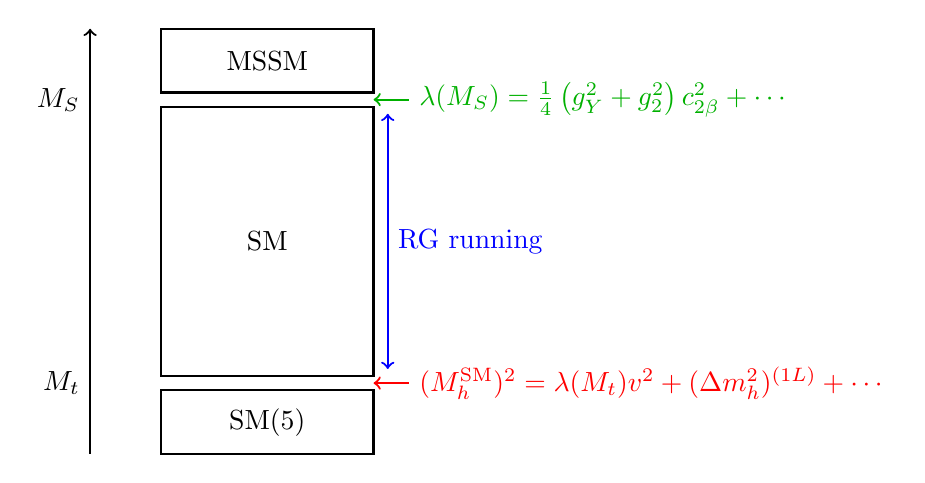
\begin{tikzpicture}[scale=0.9]
      \draw[->, thick] (0,0) -- (0,1) node[left]{$M_t$} -- (0,5) node[left]{$\MS$} -- (0,6);
      \draw[thick] (1,0)   rectangle node{SM(5)} (4,0.9);
      \draw[thick] (1,1.1) rectangle node{SM}    (4,4.9);
      \draw[thick] (1,5.1) rectangle node{MSSM}  (4,6);
      \draw[<-, thick, darkgreen] (4,5) -- (4.5,5) node[right]{$\lambda(\MS) = \frac{1}{4}\left(g_Y^{2} + g_2^2\right) c^2_{2\beta} + \cdots$};
      \draw[<-, thick, red] (4,1) -- (4.5,1) node[right]{$(M_h^\SM)^2 = \lambda(M_t) v^2 + (\Delta m_h^2)^{(1L)} + \cdots$};
      \draw[<->, thick, blue] (4.2,1.2) -- node[right]{RG running} (4.2,4.8);
    \end{tikzpicture}
  \end{center}
\end{frame}

\begin{frame}{Known/unknown loop corrections in the EFT calculation}
  \emph{SM contributions:}
  \begin{itemize}
  \item Loop corrections in the determination of the running SM
    parameters $y_f^\SM$, $g_i^\SM$:
    \begin{align*}
      y_t^\SM &= \frac{\sqrt{2}\,M_t}{v}
      \Big[1 + \hbar(\textcolor{darkgreen}{\text{full}})
      + \hbar^2(\textcolor{darkgreen}{\as^2} + \textcolor{darkgray}{\at\as} + \textcolor{darkgray}{\at^2})
      + \hbar^3(\textcolor{darkgreen}{\as^3} + \cdots)
      \Big] \\
      \as^\SM &= \as^{\SM(5)}
      \Big[1 + \hbar(\textcolor{darkgreen}{\text{full}})
      + \hbar^2(\textcolor{darkgreen}{\as^2} + \cdots)
      + \hbar^3(\textcolor{darkgreen}{\as^3} + \cdots)
      + \cdots \Big]
    \end{align*}
    \mycite{9912391, 1205.2892, 9305305, 9707474, 9708255, 0004189}
  \item Loop corrections to $M_h^2$ in the SM:
    \begin{align*}
      M_h^2 &= m_h^2 + \hbar(\textcolor{darkgreen}{\text{full}})
      + \hbar^2\Big[ m_t^2(\textcolor{darkgreen}{\at\as} + \textcolor{darkgreen}{\at^2} + \cdots)
      + \textcolor{darkgray}{m_Z^2\aem^2}
      + \cdots\Big]\\
      &\quad + \hbar^3\Big[ m_t^2(\textcolor{darkgreen}{\at\as^2} + \textcolor{darkgreen}{\at^2\as} + \textcolor{darkgreen}{\at^3})
        + \textcolor{red}{m_Z^2 \aem^3} + \cdots \Big]\\
      &\quad + \hbar^4\Big[ m_t^2(\textcolor{darkgreen}{\at\as^4} + \cdots)
      + \cdots\Big]
    \end{align*}
    \mycite{1205.6497, 1407.4336, 1508.00912}
  \end{itemize}
\end{frame}

\begin{frame}{Known/unknown loop corrections in the EFT calculation}
  \emph{SUSY contributions:} Loop corrections to $\lambda(\MS)$:
  \begin{align*}
      \lambda(\MS) &= \frac{1}{4}(g_Y^2+g_2^2)c_{2\beta}^2 + \hbar(\textcolor{darkgreen}{\text{full}}) \\
      &\quad + \hbar^2\Big[ (\textcolor{darkgreen}{\at^2\as} + \textcolor{darkgreen}{\ab^2\as}
        + \textcolor{darkgreen}{\at^2\ab} + \textcolor{darkgreen}{\at\ab^2} + \textcolor{darkgreen}{\at^3} + \cdots)
      + \textcolor{red}{\aem^3}
      + \cdots\Big]\\
      &\quad + \hbar^3\Big[ (\textcolor{darkgreen}{\underline{\at^2\as^2}} + \textcolor{red}{\at^3\as} + \textcolor{red}{\at^4})
        + \textcolor{red}{\aem^4} + \cdots \Big]
  \end{align*}
  \mycite{1407.4081, 1504.05200, 1703.08166, \underline{1807.03509}}\\[0.5em]
  \emph{Neglected contributions:} Terms of $O(v^2/\MS^2)$
\end{frame}

\begin{frame}{Effect of the 3-loop corrections to $\lambda(\MS)$}
  3-loop corrections to $\lambda(\MS)$ allow for an N$^3$LL
  resummation of strong corrections $O(\at^2\as^2)$:
  \begin{center}
    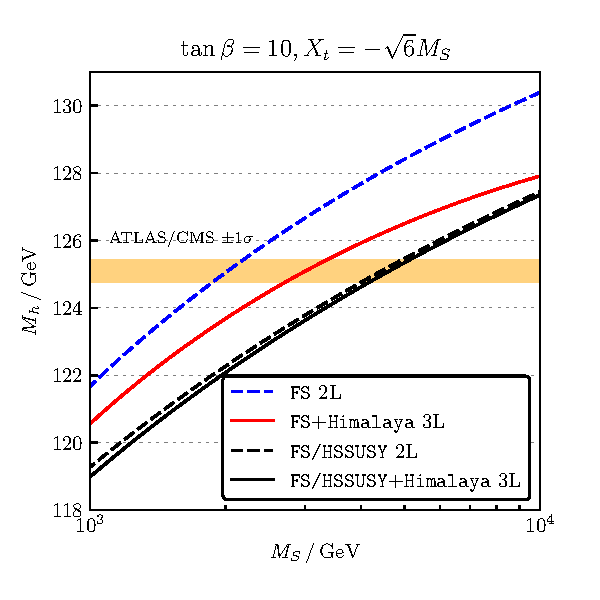
\includegraphics[width=0.49\textwidth]{plots/HSSUSY-3L/scan_Mh_MS_TB-10_Xt--sqrt6}\hfill
    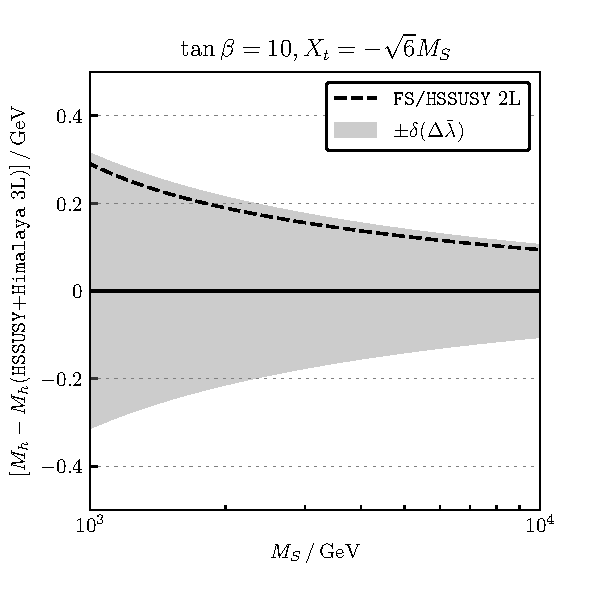
\includegraphics[width=0.49\textwidth]{plots/HSSUSY-3L/scan_Mh_MS_TB-10_Xt--sqrt6_diff}
  \end{center}
  \mycite{1807.03509}
\end{frame}

\subsection{Uncertainty estimate}

\begin{frame}{Uncertainty estimate of the EFT calculation}
  In \bigcite{1804.09410} 5 sources of uncertainty were combined:
  \begin{align*}
    \DMhQpole &= \max_{\Qpole\in[M_t/2,2M_t]}\left|M_h(\Qpole) - M_h(M_t)\right| & \text{\mycite{1609.00371}} \\
    \DMhQmatch &= \max_{\Qmatch\in[\MS/2,2\MS]}\left|M_h(\Qmatch) - M_h(\MS)\right| & \text{\mycite{1407.4081}} \\
    \DMhHSSUSYytSM &= \left| M_h(y_t^{\SM,(2L)}(M_Z)) - M_h(y_t^{\SM,(3L)}(M_Z)) \right| & \text{\mycite{1504.05200}} \\
    \DMhEFT &= \left| M_h - M_h(v^2/\MS^2) \right| & \text{\mycite{1504.05200}} \\
    \DMhHSSUSYytMSSM &= \left| M_h - M_h(y_t^\MSSM(\MS)) \right| & \text{\mycite{Bagnaschi,AV,Weiglein}}
  \end{align*}
  Combination:
  \begin{align*}
    \DMhHSSUSY &= \DMhQpole + \DMhQmatch + \DMhHSSUSYytSM + \DMhHSSUSYytMSSM \\
    &\quad + \DMhEFT
  \end{align*}
\end{frame}

\begin{frame}{Comparison of fixed-order and EFT approaches}
  \begin{center}
    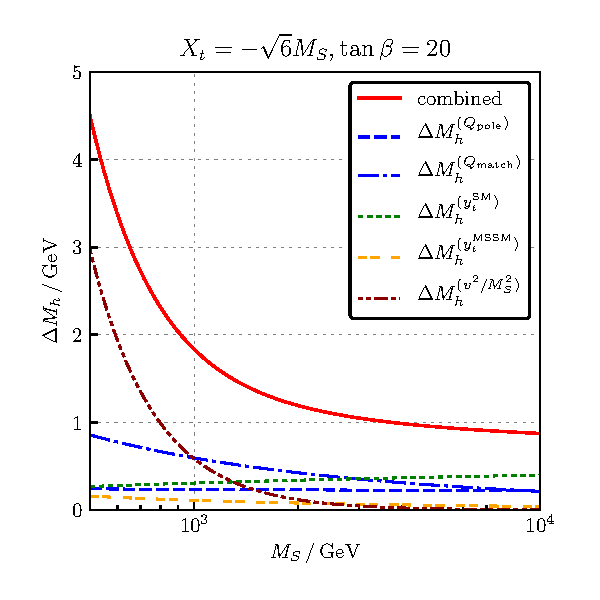
\includegraphics[width=0.49\textwidth]{plots/SOFTSUSY/HSSUSY_TB-20_Xt--sqrt6_individual}\hfill
    \includegraphics[width=0.49\textwidth]{plots/SOFTSUSY/Mh_MS_TB-20_Xt--sqrt6}
  \end{center}
  \begin{center}
    $\DMh \overset{!}{=} \DMhHSSUSY$\\[0.5em]
    $\Rightarrow$ $\MS^{\text{equal}} = 1.0$--$1.3\TeV$ for
    small/large $\tan\beta$ and/or $X_t$
  \end{center}
  \mycite{1804.09410}
\end{frame}

%%%%%%%%%%%%%%%%%%%%%%%%%%%%%%%%%%%%%%%%

\section{Hybrid fixed-order/EFT calculation}

\begin{frame}{Contents}
  \tableofcontents[
  currentsection,
  currentsubsection]  
\end{frame}

\begin{frame}{Hybrid fixed-order/EFT calculation}
  \emph{Goal:} resum large logarithms \emph{and} include suppressed
  $O(v^2/\MS^2)$ terms
  \\[2em]
  \emph{Two known approaches:}
  \begin{itemize}
  \item FeynHiggs \mycite{1312.4937, 1706.00346, 1805.00867}: Replace logs from
    fixed-order calculation by resummed logs
    \begin{align*}
      M_h^2 = (M_h^2)_{\text{fixed-order}} - (M_h^2)_{\text{logs}} + (M_h^2)_{\text{resummed logs}}
    \end{align*}
  \item FlexibleEFTHiggs \mycite{1609.00371, 1710.03760}: Incorporate
    $O(v^2/\MS^2)$ terms into $\lambda$ by using the matching
    condition
    \begin{align*}
      (M_h^2)_{\SM} \overset{!}{=} (M_h^2)_{\BSM} \qquad \text{at } Q = \MS
    \end{align*}
  \end{itemize}
\end{frame}

\begin{frame}{FlexibleEFTHiggs approach \mycite{1609.00371, 1710.03760}}
  \emph{Idea:}
  Determine $\lambda(\MS)$ from the condition
  \begin{align*}
    (M_h^2)_{\SM} \equiv \lambda(\MS) v^2 + (\Delta m_h^2)_{\SM} \overset{!}{=} (M_h^2)_{\BSM} , \qquad Q = \MS
  \end{align*}
  \begin{center}
    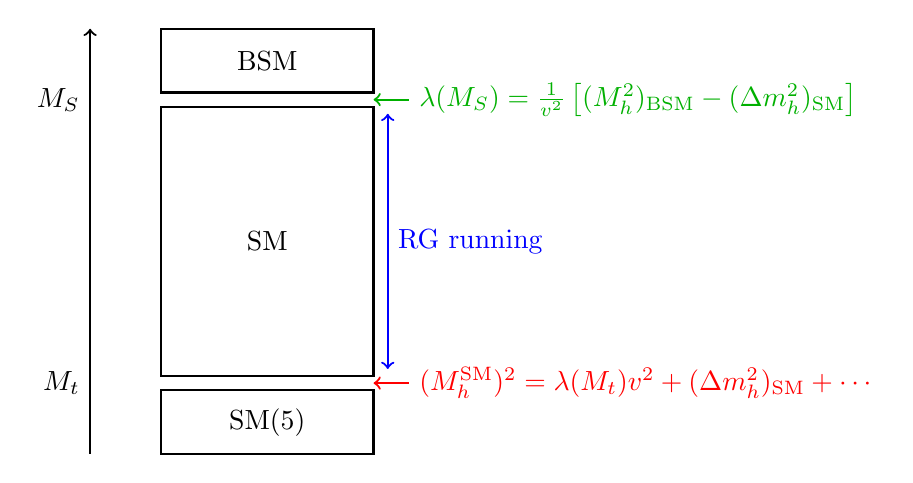
\begin{tikzpicture}[scale=0.9]
      \draw[->, thick] (0,0) -- (0,1) node[left]{$M_t$} -- (0,5) node[left]{$\MS$} -- (0,6);
      \draw[thick] (1,0)   rectangle node{SM(5)} (4,0.9);
      \draw[thick] (1,1.1) rectangle node{SM}    (4,4.9);
      \draw[thick] (1,5.1) rectangle node{BSM}  (4,6);
      \draw[<-, thick, darkgreen] (4,5) -- (4.5,5) node[right]{$\lambda(\MS) = \frac{1}{v^2}\left[(M_h^2)_{\BSM} - (\Delta m_h^2)_{\SM}\right]$};
      \draw[<-, thick, red] (4,1) -- (4.5,1) node[right]{$(M_h^\SM)^2 = \lambda(M_t) v^2 + (\Delta m_h^2)_{\SM} + \cdots$};
      \draw[<->, thick, blue] (4.2,1.2) -- node[right]{RG running} (4.2,4.8);
    \end{tikzpicture}
  \end{center}
\end{frame}

\begin{frame}{Comparison of the three approaches in the MSSM}
  Currently NLO + NLL is available \mycite{1609.00371, 1710.03760}.\\
  Extension to NNLO + NNLL is work in progress:
  \begin{center}
    \includegraphics[width=0.49\textwidth]{{{plots/FlexibleEFTHiggs-2L/Mh_MS_TB-20_Xt-0}}}
    \hfill
    \includegraphics[width=0.49\textwidth]{{{plots/FlexibleEFTHiggs-2L/Mh_MS_TB-20_Xt--sqrt6}}}
  \end{center}
  Preliminary work by Thomas Kwasnitza, Dominik Stöckinger, AV
\end{frame}

% \begin{frame}{Features FlexibleEFTHiggs approach}
%   % \begin{align*}
%   %   (M_h^2)_{\SM} &\overset{!}{=} (M_h^2)_{\BSM} \qquad \text{at } Q = \MS
%   % \end{align*}
%   \emph{Advantages:}
%   \begin{itemize}
%   \item large logarithms $\propto\ln(M_S/M_t)$ are resummed
%   \item suppressed terms $O(v^2/\MS^2)$ are incorporated in $\lambda$
%   \item can be applied to a large class of non-minimal SUSY models (NMSSM, \ESSM, MRSSM, \ldots)
%   \end{itemize}
%   \vspace{0.5em}
%   $\Rightarrow$ precise at both $\MS \sim v$ and $\MS \gg v$\\
%   \vspace{1em}
%   \emph{Limitations:}
%   \begin{itemize}
%   \item currently restricted to the SM as EFT
%   \item 2-loop suppressed terms of the form
%     $\frac{1}{(4\pi)^4}\frac{v^2}{\MS^2}\times\log(\MS/M_t)$ are
%     included, but not resummed
%   \end{itemize}
%   \emph{Disadvantage:}
%   \begin{itemize}
%   \item tricky to extend to 2-loop accuracy (work in progress)
%   \end{itemize}
% \end{frame}

\begin{frame}{Comparison in the NMSSM}
  \begin{center}
    \includegraphics[width=0.4\textwidth]{{{plots/NMSSMEFTHiggs/DMh_MS_TB-5_Xt-0_lam-0.1_kap-0.1}}}%\hfill
    \includegraphics[width=0.4\textwidth]{{{plots/NMSSMEFTHiggs/DMh_MS_TB-5_Xt-0_lam-0.3_kap-0.3}}}\\
    \includegraphics[width=0.4\textwidth]{{{plots/NMSSMEFTHiggs/DMh_MS_TB-5_Xt--2_lam-0.1_kap-0.1}}}%\hfill
    \includegraphics[width=0.4\textwidth]{{{plots/NMSSMEFTHiggs/DMh_MS_TB-5_Xt--2_lam-0.3_kap-0.3}}}
  \end{center}
\end{frame}

%%%%%%%%%%%%%%%%%%%%%%%%%%%%%%%%%%%%%%%%

\section{Summary}

\begin{frame}{Summary}
  \emph{Supersymmetry} is still viable, but
  \begin{itemize}
  % \item LHC continuously excludes light SUSY scenarios with
  %   $\MS \lesssim 1\TeV$
  \item $\MS \gtrsim 1\TeV$ required in the MSSM to predict
    $M_h = 125.09\GeV$
  \end{itemize}
  %
  \vspace{1em}
  \emph{Recent advances in the calculation of $M_h$ in the MSSM:}
  \begin{itemize}
  \item fixed-order (\DRbarp): 3-loop $O(\at\as^2)$ correction to $M_h$
  \item EFT (single-scale): 3-loop $O(\at\as^2)$ correction to $\lambda$ \\
    $\rightarrow$ N$^3$LL resummation of strong corrections
  \item hybrid (FlexibleEFTHiggs): NLO + NLL available, \\
    NNLO + NNLL comming soon
  \end{itemize}
  %
  \vspace{1em}
  \emph{When to use the MSSM \DRbarp\ fixed-order/EFT calculation?}
  \begin{itemize}
  \item $\MS \lesssim 1\TeV$ $\Rightarrow$ use fixed-order
  \item $\MS \gtrsim  1\TeV$ $\Rightarrow$ use EFT
  \end{itemize}
\end{frame}

%%%%%%%%%%%%%%%%%%%%%%%%%%%%%%%%%%%%%%%%

\begin{frame}{Current status of (N)MSSM spectrum generators}
  \begin{center}
    \emph{MSSM}\\[0.4em]
    \begin{tabular}{llll}
      \toprule
      Spectrum generator & fixed order & EFT & hybrid \\
      \midrule
      \FH                & 2L & 2L & NNLO + NNLL \\
      \FS                & \textcolor{darkgreen}{3L} & \textcolor{darkgreen}{3L} & \textcolor{darkgreen}{NNLO + NNLL}$^\dagger$ \\
      \SOFTSUSY          & \textcolor{darkgreen}{3L} & -- & -- \\
      \SARAH/\SPheno     & 2L & -- & NNLO + LL \\
      \bottomrule
    \end{tabular}
  \end{center}
  %
  \begin{center}
    \emph{NMSSM}\\[0.4em]
    \begin{tabular}{llll}
      \toprule
      Spectrum generator & fixed order & EFT & hybrid \\
      \midrule
      \FH                & -- & -- & -- \\
      \FS                & 2L$^*$ & -- & \textcolor{darkgreen}{NNLO + NNLL}$^\dagger$ \\
      \SOFTSUSY          & 2L$^*$ & -- & -- \\
      \SARAH/\SPheno     & 2L & -- & NNLO + LL \\
      \bottomrule
    \end{tabular}
  \end{center}
  $^\dagger$: not released yet\\
  $^*$: $O(\at^2)$ corrections in the MSSM limit, no $O(\at\lambda^2)$ corrections
\end{frame}

%%%%%%%%%%%%%%%%%%%%%%%%%%%%%%%%%%%%%%%%
% backup slides
%%%%%%%%%%%%%%%%%%%%%%%%%%%%%%%%%%%%%%%%

\begin{frame}[noframenumbering]
  \begin{center}
    \Huge Backup
  \end{center}
\end{frame}

%%%%%%%%%%%%%%%%%%%%%%%%%%%%%%%%%%%%%%%%

\begin{frame}[noframenumbering]{Uncertainty estimate of the fixed-order \DRbarp\ calculation}
  Calculation of $m_t$ in two different ways as proposed in
  \bigcite{1609.00371}:
  \begin{align*}
    m_t^{[1]} &=
                M_t + \widetilde{\Sigma}_t^{(1L),S} +
                M_t \left[
                \widetilde{\Sigma}_t^{(1L),L} +
                \widetilde{\Sigma}_t^{(1L),R}
                \right] \\
              &\phantom{={}} + M_t
                \left[\widetilde{\Sigma}_t^{(1L),\SQCD}
                + \widetilde{\Sigma}_t^{(2L),\SQCD}
                + \left(\widetilde{\Sigma}_t^{(1L),\SQCD}\right)^2
                \right]\\
    m_t^{[2]} &=
                M_t + \widetilde{\Sigma}_t^{(1L),S} +
                m_t \left[
                \widetilde{\Sigma}_t^{(1L),L} +
                \widetilde{\Sigma}_t^{(1L),R}
                \right] \nonumber \\
              &\phantom{={}} +
                m_t
                \left[\widetilde{\Sigma}_t^{(1L),\SQCD} +
                \widetilde{\Sigma}_t^{(2L),\SQCD}
                \right]
  \end{align*}
  Calculation of $\as$ and $\aem$ in two different ways:
  \begin{align*}
    \as^{[1]}  &= \frac{\as^{\SM(5)}}{1 - \Delta^{(1L)}\as - \Delta^{(2L)}\as}\\
    \as^{[2]}  &= \as^{\SM(5)} \left[1 + \Delta^{(1L)}\as + (\Delta^{(1L)}\as)^2 + \Delta^{(2L)}\as\right]
  \end{align*}
\end{frame}

%%%%%%%%%%%%%%%%%%%%%%%%%%%%%%%%%%%%%%%%

\begin{frame}[noframenumbering]{Uncertainty estimate of FlexibleEFTHiggs-1L}
  \begin{align*}
    \DMhQpole &= \max_{\Qpole\in[M_t/2,2M_t]}\left|M_h(\Qpole) - M_h(M_t)\right| & \text{\mycite{1609.00371}} \\
    \DMhQmatch &= \max_{\Qmatch\in[\MS/2,2\MS]}\left|M_h(\Qmatch) - M_h(\MS)\right| & \text{\mycite{1407.4081}} \\
    \DMhHSSUSYytSM &= \left| M_h(y_t^{\SM,(2L)}(M_Z)) - M_h(y_t^{\SM,(3L)}(M_Z)) \right| & \text{\mycite{1504.05200}} \\
    \DMhEFT &= 0 \quad \text{(has no EFT uncertainty!)} & \text{\mycite{1609.00371}}
  \end{align*}
\end{frame}

\end{document}
